\label{sec:self-advection-implementation}
Where more renowned methods of solving differential equations are failing to find a numerical solution to eq. (\ref{eq:self-advect}) (such as forward Euler for the time derivative and central difference for the spatial derivative\footnote{Which is unconditionally unstable for any \begin{math}\Delta t\end{math} \cite[p.~28]{bridson}}), a method called semi-Lagrangian method is often used to ensure unconditional stability. As the name implies, it is motivated by taking a Lagrangian viewpoint (which treats the fluid as a set of finite particles) in order to aid the Eulerian grid based approach. Consider a particle at  \begin{math}\vec{x}\end{math}, with velocity \begin{math}\vec{u}(\vec{x}) = \frac{d\vec{x}}{dt}\end{math}. If the particle started from grid location \begin{math}\vec{x}_G\end{math} and ended up at \begin{math}\vec{x}_P\end{math} after time step \begin{math}\Delta t \end{math}, assuming constant velocity we have that: 
\begin{equation}
\label{eq:lagrangian-arg}
\vec{u}(t,\vec{x}_G) = \vec{u}(t+\Delta t,\vec{x}_P)  
\end{equation}
The same argument can be made backwards: there exists a particle at \begin{math}\vec{x}_{P_1} \end{math} that will end up at grid location \begin{math}\vec{x}_{G_1}\end{math}, finding \begin{math}\vec{x}_{P_1}\end{math} is done simply by tracing the current velocity field backwards in time and evaluating the velocity field at that point. Using simple Euler integration gives: 
%\begin{equation}
	\begin{align}
					      \label{eq:lagrangian}\vec{x_{P_1}}  & =    \vec{x_{G_1}} -  \Delta t \vec{u}(\vec{x_{G_1}})  \\ 
		\label{eq:lagrangian-arg-reverse}\vec{u}(t + \Delta t,\vec{x}_{G_1}) &  =    \vec{u}(t,\vec{x}_{P_1}) 
	\end{align}
%\end{equation}
\begin{math} \vec{x_{P_1}} \end{math} is not very likely to be directly at a known grid point, so in order to find \begin{math} \vec{u}(\vec{x_{P_1}}) \end{math} some kind of interpolation has to be used. Trilinear interpolation is prone to smooth the velocity field and better alternatives exists, such as Catmull-Rom interpolation, which reduces the dissipation (smoothing) and boosts the accuracy to second order (trilinear has first order accuracy). Despite the shortcomings of trilinear interpolation it showed to be adequate for convincing visual results.

\subsubsection{Practical example in 2D}
Below is a simplified 2D illustration to further illustrate the advection update of a velocity vector (e.q (\ref{eq:lagrangian-arg})-(\ref{eq:lagrangian-arg-reverse})) as well as a quick look at the bilinear-interpolation of the face-vectors. To extrapolate this to the third dimension trilinear interpolation has to be used in step 1 (fig. \ref{fig:bilinear-interpolation}) instead of bilinear interpolation. 
\begin{figure}[H]
\centering
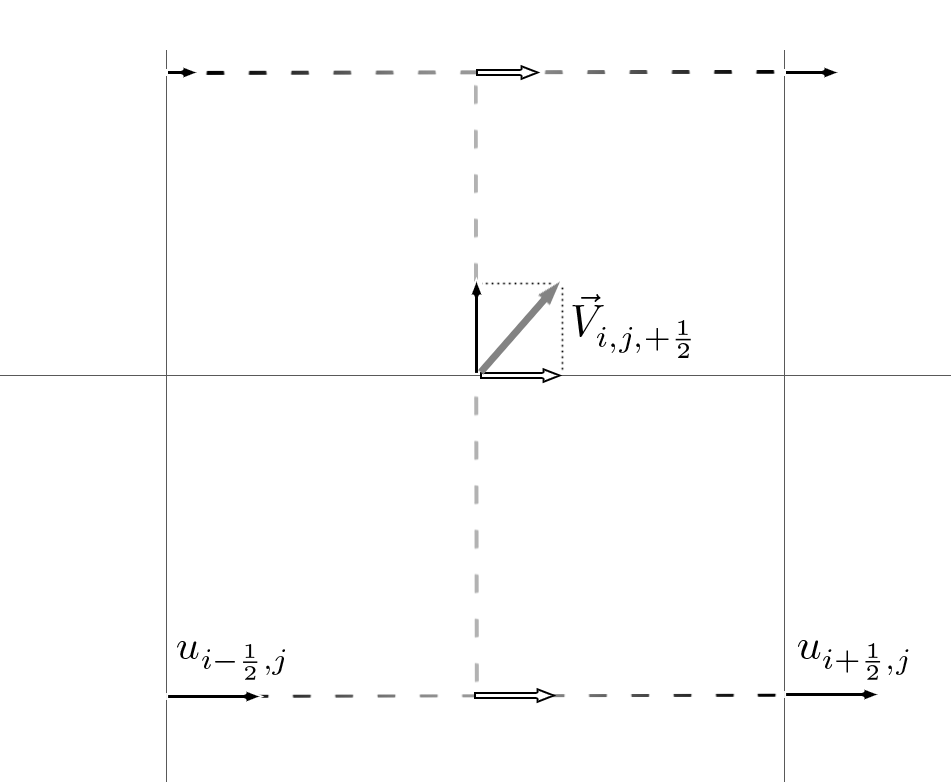
\includegraphics[width=0.75\textwidth]{semi-lagrangian-grid-interpolate.png}
\caption{To find $\vec{V}_{i,j+\frac{1}{2}}$ linear interpolation is used on the $v$ components. Black arrows represent known scalar values and white arrows represent interpolated values. Keep in mind that they are implicitly known to be vectors, not stored as such. The gray vector in the center $\vec{V}_{{i}{j+\frac{1}{2}}}$ is the vector found by combining the interpolated u-component and the explicitly known v component.}
\label{fig:bilinear-interpolation}
\end{figure}

\begin{figure}[H]
\centering
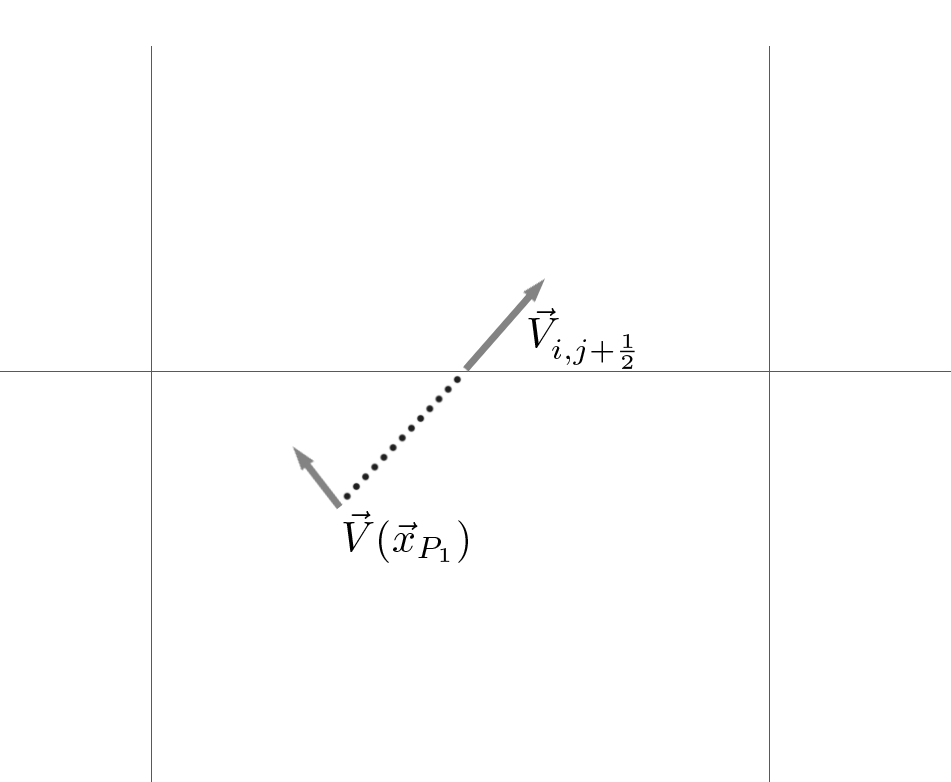
\includegraphics[width=0.75\textwidth]{semi-lagrangian-grid-backwards.png}
\caption{Once the location $\vec{x}_{P_1}$ is found by tracing backwards from $\vec{x}_{i,j+\frac{1}{2}}$ ($\vec{x}_{P_1} = \vec{x}_{i,j+\frac{1}{2}}-\Delta x \vec{V}_{i,j+\frac{1}{2}}$) as described in section \ref{sec:self-advection-implementation}. The vector $\vec{V}(\vec{x}_{P_1})$ is acquired by interpolating the nearby $u$ and $v$ components as in fig \ref{fig:bilinear-interpolation} }
\end{figure}

\begin{figure}[H]
\centering
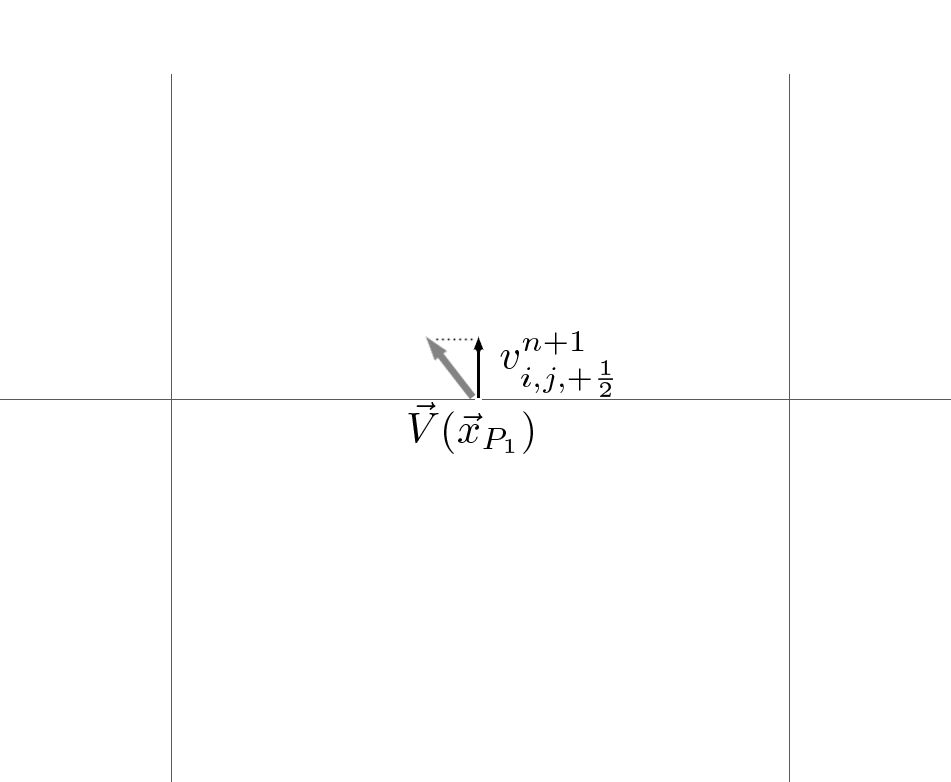
\includegraphics[width=0.75\textwidth]{semi-langrangian-grid-update.png}
\caption{When $\vec{V}(\vec{x}_{P_1})$ is found the next time step can be updated as: $v^{n+1}_{i,j+\frac{1}{2}} = \vec{V}(\vec{x}_{P_1})_{v} $}
\end{figure}
